\section{Arithmetic Programs}
Suppose we have some algebra \(\mathbb{A}\): we can represent and deal with finite sequences of 
operations, called \emph{expressions}, between elements of \(\mathbb{A}\) and/or variables over 
\(\mathbb{A}\).

For example, given the expression \(x^2 + x + 1\) over \(\extend{\mathbb{A}}{x}\), we might be 
interested to know what is the \emph{evaluation} of the expression given some value for \(x\).
We will limit our analysis to fields (and rings).
\begin{definition}[Arithmetic formula over a field]
  Given a field \(\mathbb{F}\), an \emph{explicit arithmetic formula} over \(\mathbb{F}\) is any 
  expression \(\varphi \) of the kind:
  \begin{align*}
    & \varphi \equiv a && \textnormal{with \(a\) constant over \(\mathbb{F}\)} \\ 
    & \varphi \equiv x && \textnormal{with \(x\) variable over \(\mathbb{F}\)} \\
    & \varphi \equiv \varphi_1 \oplus \varphi_2 && 
    \textnormal{with \(\varphi_1, \varphi_2\) formulae over \(\mathbb{F}\)} \\
    & \varphi \equiv \varphi_1 \otimes \varphi_2 && 
    \textnormal{with \(\varphi_1, \varphi_2\) formulae over \(\mathbb{F}\)}
  \end{align*}
  Additionally, an \emph{implicit arithmetic formula} also allows expressions involving 
  exponentiations:
  \begin{align*}
    & \varphi \equiv \varphi_{1}^{k} && 
    \textnormal{\(\forall k \in \mathbb{N}\), with \(\varphi_1\) formula over \(A\)}
  \end{align*}
\end{definition}

It is always possible to translate an implicit formula into an equivalent explicit one by unrolling 
exponentiations.
We denote the explicit version of an implicit formula \(\varphi \) with \(\explicit{\varphi}\).
Note also that multiplication by constants can also be unrolled to a sequence of additions 
(in fact, they can be viewed as exponentiations w.r.t.\ addition).
From now on, we will only deal with arithmetic formulae over some field (or ring) \(\mathbb{F}\), 
in which case implicit arithmetic expressions are equivalent to multi-variate polynomials.
\begin{example}\label{ex:arithmetic_formula}
  Consider the finite field \(\mathbb{Z}_{13}\).
  For ease of notation, we will use \(+\), juxtaposition and superscripting to denote, respectively,
  field addition, field multiplication, and exponentiation w.r.t.\ field multiplication. 
  A possible implicit arithmetic formula over \(\mathbb{Z}_{13}\) is the following expression:
  \[\varphi = x_{2}\Parens*{x_{1}^{3} + 4x_{2} + 5}\]
  Since in a finite field multiplication by a constant is simply repeated addition, i.e. 
  \(cx = \call{+^{c}}{x}\), the explicit version of \(\varphi \) then is:
  \[\explicit{\varphi} = x_{2}\Parens*{x_{1}x_{1}x_{1} + x_{2} + x_{2} + x_{2} + x_{2} + 5}\]
\end{example} 

\subsection{Arithmetic circuits}
It is possible to visually represent an arithmetic formula using a particular kind of labeled 
\emph{directed acyclic graph} (DAG), called the \emph{arithmetic circuit}.
\begin{definition}[Arithmetic circuit]
  An \emph{arithmetic circuit} over a field \(\mathbb{F}\) and a set of variables \(X\) over 
  \(\mathbb{F}\) is a triple \(\mathcal{G} = \Tuple{V, E, L}\) where 
  \(V\) is the set of \emph{vertices}, \(E \subseteq V \times V\) is the set of \emph{edges}, and 
  \(L\colon V \to A \cup X \cup \Parens*{\Set{\oplus, \otimes} \times \mathbb{N}}\) is 
  the vertex \emph{labeling map}, such that, \(\forall v \in V\):
  \begin{align*}
    & \call{L}{v} \in A && \implies \nexists w \in V\colon \Tuple{w, v} \in E
    && \textnormal{(no in-edges for constant nodes)} \\
    & \call{L}{v} \in X && \implies \nexists w \in V\colon \Tuple{w, v} \in E
    && \textnormal{(no in-edges for variable nodes)} \\
    & \forall \odot_i \in \call{L}{v} && \implies \abs{\Set{\Tuple{w, v}}_{w \in V} \cap E} = 
    \abs{\odot} && \textnormal{(exactly \(\abs{\odot}\) in-edges for \(\odot_i\) nodes)} \\
  \end{align*}
\end{definition}

As an abuse of notation, we will sometimes identify a node \(v\) with its label \(\call{L}{v}\).
Given any explicit arithmetic formula \(\varphi \) over an algebra \(\mathbb{A}\) and a set of 
variables \(X\), we can build the corresponding arithmetic circuit \(\mathcal{G} = \Tuple{V, E, L}\) 
in the following way: for every distinct (i.e.\ ignoring repetitions) variable \(x\) appearing 
in \(\varphi \), we add a vertex \(v\) with label \(\call{L}{v} = x\); 
for every distinct constant \(c\) appearing in \(\varphi \) we add a vertex \(v\) with label 
\(\call{L}{v} = c\); 
finally, for every occurrence \(i\) of some operation \(\odot \) in \(\varphi \), we add a vertex
\(v\) with label \(\call{L}{v} = \odot_{i}\).
We can partition \(V\) as follows:
\begin{itemize}
  \item \emph{Constant vertices}: 
    \(\mathcal{G}_{const} = \Set{v \mid \call{L}{v} \in \mathbb{F}}\).
  \item \emph{Variable vertices}: 
    \(\mathcal{G}_{var} = \Set{v \mid \call{L}{v} \in X}\).
  \item \emph{Addition vertices}: 
    \(\mathcal{G}_{\oplus} = \Set{v \mid \oplus \in \call{L}{v}}\).
  \item \emph{Multiplication vertices}: 
    \(\mathcal{G}_{\otimes} = \Set{v \mid \otimes \in \call{L}{v}}\).
    \item \emph{Operation vertices}:
    \(\mathcal{G}_{\odot} = \mathcal{G}_{\oplus} \cup \mathcal{G}_{\otimes}\).
  \item \emph{Input vertices}: 
    \(\mathcal{G}_{in} = \mathcal{G}_{const} \cup \mathcal{G}_{var}\).
  \item \emph{Output vertices}: 
    \(\mathcal{G}_{out} = \Set{v \mid \nexists w \in V\colon \Tuple{v, w} \in E}\).
  \item \emph{I/O vertices}: \(\mathcal{G}_{IO} = \mathcal{G}_{in} \cup \mathcal{G}_{out}\).
\end{itemize}

To build the set of edges \(E\), for every operation occurring in \(\varphi \), we connect the 
vertices representing the operands to the vertex representing said operation, e.g.\ if we have 
the formula \(\Parens*{x \odot y} \odot z\) we add the edges \(\Tuple{x, \odot_1}\), 
\(\Tuple{y, \odot_1}\) and \(\Tuple{z, \odot_2}\).
We also consider operation nodes as holding the intermediate values of the computation: in the 
previous example, we will also have the edge \(\Tuple{\odot_1, \odot_2}\), where \(\odot_1 \) 
represents the intermediate value \(x \odot y\).
The fact that we store all the intermediate values of a computation can be greatly exploited when
optimizing the design of a circuit for some formula.

Since arithmetic circuits contain no cycles, they can only be used to represent a fixed number 
of operations (aka \emph{bounded computations}).
In general though, this is not really a big issue, as oftentimes we can easily synthesize circuits 
\emph{on-the-fly}.

\begin{example}\label{ex:arithmetic_circuit}
  \Cref{fig:arithmetic_circuit} shows the arithmetic circuit derived from the formula shown in 
  \Cref{ex:arithmetic_formula}.
  We can see the two variable vertices \(x_1\) and \(x_2\) which are also input vertices, the 
  constant vertex \(5\), which is an input vertex too, the
  addition vertices \(\oplus_1, \dots, \oplus_5\) and the multiplication vertices 
  \(\otimes_1, \otimes_2, \otimes_3\), of which the latter is also an output vertex.
\end{example}

\begin{figure}
	\centering
	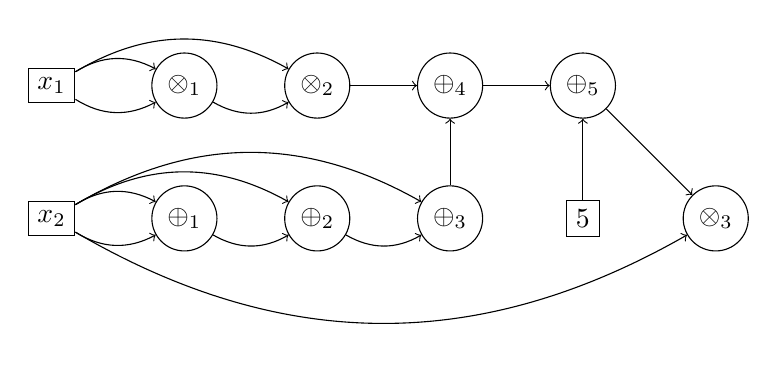
\begin{tikzpicture}[node distance={48pt}, node/.style = {draw, circle}]
		\node[node,shape=rectangle] (x1) {\(x_1\)};
		\node[node,shape=rectangle] (x2) [below of=x1] {\(x_2\)};
		\node[node] (m1) [right of=x1] {\(\otimes_1\)};
		\node[node] (m2) [right of=m1] {\(\otimes_2\)};
		\node[node] (a1) [right of=x2] {\(\oplus_1\)};
		\node[node] (a2) [right of=a1] {\(\oplus_2\)};
		\node[node] (a3) [right of=a2] {\(\oplus_3\)};
		\node[node] (a4) [right of=m2] {\(\oplus_4\)};
		\node[node] (a5) [right of=a4] {\(\oplus_5\)};
		\node[node,shape=rectangle] (5) [below of=a5] {\(5\)};
		\node[node] (m3) [right of=5] {\(\otimes_3\)};
		\draw[->] (x1) to [bend left] (m1);
		\draw[->] (x1) to [bend right] (m1);
		\draw[->] (x1) to [bend left] (m2);
		\draw[->] (m1) to [bend right] (m2);
		\draw[->] (x2) to [bend left] (a1);
		\draw[->] (x2) to [bend left] (a2);
		\draw[->] (x2) to [bend left] (a3);
		\draw[->] (x2) to [bend right] (a1);
		\draw[->] (a1) to [bend right] (a2);
		\draw[->] (a2) to [bend right] (a3);
		\draw[->] (m2) to (a4);
		\draw[->] (a3) to (a4);
		\draw[->] (a4) to (a5);
		\draw[->] (5) to (a5);
		\draw[->] (a5) to (m3);
		\draw[->] (x2) to [bend right] (m3);

	\end{tikzpicture}
	\caption{Circuit of the formula in \Cref{ex:arithmetic_formula}. 
  Rectangular nodes represent input vertices.}\label{fig:arithmetic_circuit}
\end{figure}

\begin{definition}[Circuit input]
  A \emph{circuit input} for an arithmetic circuit \(\mathcal{G} = \Tuple{V, E, L}\) over a 
  field \(\mathbb{F}\) is a triple \(\mathcal{I}_{\mathcal{G}} = \Tuple{V, E, L'}\) such that, 
  \(\forall v \in \mathcal{G}_{in}\colon \call{L'}{v} \in \mathbb{F}\).
\end{definition}

In particular, since every vertex in \(G_{in}\) has now a constant value, \(\mathcal{I}\) induces 
an \emph{evaluation} \(\mathcal{E}\) over \(\mathcal{G}\) which associates to every operation vertex 
\(v \in \mathcal{G}_{\odot}\) the value \(\call{\eval}{v}\). 
\begin{definition}[Circuit assignment]
  A \emph{circuit assignment} for an arithmetic circuit \(\mathcal{G} = \Tuple{V, E, L}\) over a 
  field \(\mathbb{F}\) is a triple \(\mathcal{A}_{\mathcal{G}} = \Tuple{V, E, L'}\) such that, 
  \(\forall v \in V\colon \call{L'}{v} \in \mathbb{F}\).
\end{definition}

An assignment \(\mathcal{A}\) for a circuit \(\mathcal{G}\) associates to every node of the circuit 
a value over the underlying field, but not necessarily a sensible one.
However, as an assignment is also a circuit input, it induces an evaluation.
Therefore, we say that \(\mathcal{A}\) is \emph{valid} if and only if 
\(\call{L'}{v} = \call{\eval}{v}\).

\begin{example}\label{ex:arithmetic_eval}
  \Cref{fig:circuit_assign_ok} shows a valid assignment for the circuit \(\mathcal{G}\) 
  shown in \Cref{ex:arithmetic_circuit}: we fix the inputs \(x_1 = 2\) and \(x_2 = 3\), and label 
  every operation vertex \(v\) with the correct value \(\call{\eval}{v}\).
\end{example}

\begin{figure}
	\centering
	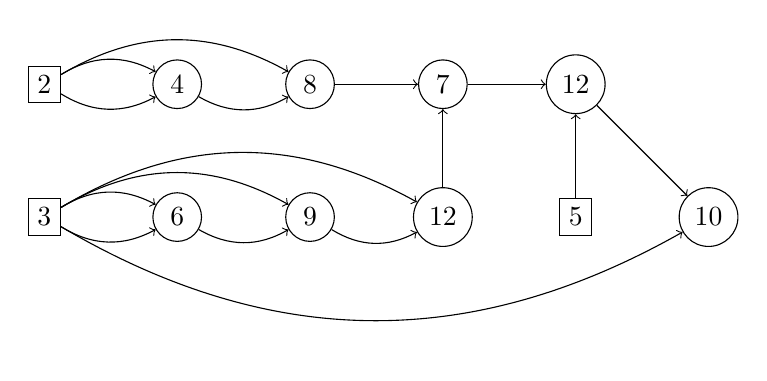
\begin{tikzpicture}[node distance={48pt}, node/.style = {draw, circle}]
		\node[node,shape=rectangle] (x1) {\(2\)};
		\node[node,shape=rectangle] (x2) [below of=x1] {\(3\)};
		\node[node] (m1) [right of=x1] {\(4\)};
		\node[node] (m2) [right of=m1] {\(8\)};
		\node[node] (a1) [right of=x2] {\(6\)};
		\node[node] (a2) [right of=a1] {\(9\)};
		\node[node] (a3) [right of=a2] {\(12\)};
		\node[node] (a4) [right of=m2] {\(7\)};
		\node[node] (a5) [right of=a4] {\(12\)};
		\node[node,shape=rectangle] (5) [below of=a5] {\(5\)};
		\node[node] (m3) [right of=5] {\(10\)};
		\draw[->] (x1) to [bend left] (m1);
		\draw[->] (x1) to [bend right] (m1);
		\draw[->] (x1) to [bend left] (m2);
		\draw[->] (m1) to [bend right] (m2);
		\draw[->] (x2) to [bend left] (a1);
		\draw[->] (x2) to [bend left] (a2);
		\draw[->] (x2) to [bend left] (a3);
		\draw[->] (x2) to [bend right] (a1);
		\draw[->] (a1) to [bend right] (a2);
		\draw[->] (a2) to [bend right] (a3);
		\draw[->] (m2) to (a4);
		\draw[->] (a3) to (a4);
		\draw[->] (a4) to (a5);
		\draw[->] (5) to (a5);
		\draw[->] (a5) to (m3);
		\draw[->] (x2) to [bend right] (m3);

	\end{tikzpicture}
	\caption{A valid assignment for the circuit in \Cref{fig:arithmetic_circuit}. 
  Remember that the underlying field is \(\mathbb{Z}_{13}\).}\label{fig:circuit_assign_ok}
\end{figure}

\subsection{Rank-1 Constraint Systems}
An arithmetic circuit tells us two things:
\begin{enumerate*}[label=(\roman*)] %chktex 36
  \item how to compute the intermediate values, after fixing the inputs, and
  \item  how the intermediate values are constrained, depending on the inputs.
\end{enumerate*}   
\begin{definition}[Rank-1 Contraint System~\cite{CramerD1998}]
	Given \(m,n \in \mathbb{N}\), an \emph{\(m/n\) Rank-1 Constraint System (R1CS)} over a field 
	\(\mathbb{F}\) is a triple \(\mathcal{C} = \Tuple{\bm{A}, \bm{B}, \bm{C}}\) such that 
  \(\bm{A}, \bm{B}, \bm{C} \in \mathbb{F}^{m \times n}\).
\end{definition}
\begin{definition}[R1CS solution]
  A \emph{solution} to an R1CS \(\mathcal{C}\) over a field \(\mathbb{F}\) is a vector 
  \(\bm{s} \in \mathbb{F}^n\) such that 
  \(\Parens*{\bm{A}\bm{s}}\Parens*{\bm{B}\bm{s}} = \bm{C}\bm{s}\).
\end{definition}
Any explicit arithmetic circuit \(\mathcal{G}\) with \(m\) multiplicative gates 
(i.e.\  \(m = \abs{\mathcal{G}_{\otimes}}\)) and \(n\) input variables 
(i.e.\  \(n = \abs{\mathcal{G}_{var}}\)) can be associated with an \({m}/\Parens*{n+m+1}\) 
R1CS \(\mathcal{C}\) representing the constraints in the circuit, as follows:
\begin{enumerate}
	\item Add a new `constant variable' \(x_0\) which always assumes value \(1\).
	\item For every multiplicative gate \(\otimes_i \) in the circuit, add a new \emph{intermediate}
	      variable \(t_i\). 
	\item Define the column vector
	      \(\bm{x} = {\begin{pmatrix}1 & x_1 & \cdots & x_n & t_1 & \cdots & t_m \end{pmatrix}}^\transpose \).
	\item Express every multiplication gate \(\otimes_i \) as an equation in the canonical form
	      \(\Parens*{\bm{A}_i\bm{x}}\Parens*{\bm{B}_i\bm{x}} = \bm{C}_i\bm{x}\).
\end{enumerate}

The intermediate variable \(t_m\), which corresponds to the `last' multiplication gate, is often 
denoted \(y\) as it represents the output of the circuit.
\begin{example}\label{ex:r1cs}
	Consider the circuit of \Cref{ex:arithmetic_circuit}: there are three multiplications in total, 
  and since we have two input variables, the associated R1CS \(\mathcal{C}\) will be a \(3/6\) 
  R1CS\@.
	So, our variable vector will be:
	\[\bm{x} = {\begin{pmatrix}1 & x_1 & x_2 & t_1 & t_2 & y\end{pmatrix}}^{\transpose}\]
  Let us explicit all the intermediate variables, and transform the constraint equations in 
  canonical form:
	\begin{align*}
		 & {t_1 = x_1x_1} && \iff && {\Parens*{x_1}\Parens*{x_1} = t_1} \\ 
     & {t_2 = t_1x_1 + 4x_2 + 5} && \iff && {\Parens*{t_1}\Parens*{x_1} = 8 + 9x_2 + t_2}\\
     & {y = t_2x_2} && \iff && {\Parens*{x_2}\Parens*{t_2} = y}
	\end{align*}
	We can now extract the \(\bm{A}\), \(\bm{B}\), \(\bm{C}\) matrices:
	\begin{align*}
    &
		\bm{A} =
		\begin{pmatrix}
      0 & 1 & 0 & 0 & 0 & 0 \\
      0 & 0 & 0 & 1 & 0 & 0 \\
      0 & 0 & 0 & 0 & 1 & 0
    \end{pmatrix}
    &&
    \bm{B} =
		\begin{pmatrix}
      0 & 1 & 0 & 0 & 0 & 0 \\
      0 & 1 & 0 & 0 & 0 & 0 \\
      0 & 0 & 1 & 0 & 0 & 0
    \end{pmatrix}
    &&
    \bm{C} =
		\begin{pmatrix}
				0 & 0 & 0 & 1 & 0 & 0 \\
				8 & 0 & 9 & 0 & 1 & 0 \\
				0 & 0 & 0 & 0 & 0 & 1
			\end{pmatrix}
  \end{align*}
  Let's check the assignment that was given in \Cref{ex:arithmetic_eval}, where \(x_1 = 2\) and 
  \(x_2 = 3\):
	\begin{align*}
		 & t_1 = x_1x_1 = 2 \times 2 = 4                              &  & \equiv  4 \pmod{13} \\
		 & t_2 = t_1x_1 + 4x_2 + 5 = 4 \times 2 + 4 \times 3 + 5 = 25 &  & \equiv 12 \pmod{13} \\
		 & y = t_2x_2 = 12 \times 3 = 36                              &  & \equiv 10 \pmod{13}
	\end{align*}
	The solution vector \(\bm{s}\) will be:
	\[\bm{s} = {\begin{pmatrix}1 & 2 & 3 & 4 & 12 & 10\end{pmatrix}}^{\transpose} \]
	It is not hard to verify that indeed
	\(\Parens*{\bm{A}\bm{s}}\Parens*{\bm{B}\bm{s}} = \bm{C}\bm{s}\).
\end{example}

\subsection{Quadratic Arithmetic Programs}\label{subsec:qap}
The size of a solution for a R1CS grows linearly in the number of multiplication gates of
the corresponding arithmetic circuit.
This is an issue, as such solution is not \emph{compact}: by compact, we mean that its size 
should be constant (i.e.\ independent of the circuit's size) or at most logarithmic (i.e.\ 
upper-bounded by a logarithmic function in the circuit's size).
\begin{definition}[Quadratic Arithmetic Program~\cite{GennaroGPR2012}]
	Given some \(m,n \in \mathbb{N}\), an
	\emph{\(m/n\) Quadratic Arithmetic Program (QAP)} over \(\mathbb{F}\) is a quadruple
	\(\mathcal{Q} = \Tuple{t, \bm{v}, \bm{w}, \bm{y}}\) where \(t \in \extend{\mathbb{F}}{x}\) is 
  the \emph{target} polynomial, and \(\bm{v}, \bm{w}, \bm{y} \in \extend{\mathbb{F}}{x}^m\) are,
  respectively, the \emph{left input polynomial}, the \emph{right input polynomial} and the 
  \emph{output polynomial}, such that:
	\[\forall i \le m\colon \call{\deg}{\bm{v}_i} = \call{\deg}{\bm{w}_i} = \call{\deg}{\bm{y}_i} 
	= \call{\deg}{t} - 1 = n - 1\]
	%A \emph{valid assignment} to a QAP \(\mathcal{Q}\) is a vector 
	%\(\bm{s} \in \mathbb{F}^m\) such that 
	%\(\Parens*{\bm{v}\bm{s}}\Parens*{\bm{w}\bm{s}} - \Parens*{\bm{y}\bm{s}} \bmod t = 0\).
	%The polynomials \(p = \Parens*{\bm{v}\bm{s}}\Parens*{\bm{w}\bm{s}} - \bm{y}\bm{s}\)
	%and \(h = p/t\) are a \emph{solution} to \(\mathcal{Q}\).
\end{definition}
\begin{definition}[QAP solution]
	A \emph{solution} to a QAP \(\mathcal{Q} = \Tuple{t, \bm{v}, \bm{w}, \bm{y}}\) over a field 
	\(\mathbb{F}\) is a pair of polynomials \(h,p \in \extend{\mathbb{F}}{x}\) such that \(p = ht\).
\end{definition}

It is possible to represent any \(m/n\) R1CS \(\mathcal{C}\) with an \(m/n\) QAP \(\mathcal{Q}\).
First, we choose any arbitrary row vector \(\bm{z} \in \Parens*{\mathbb{F}^m}^{\transpose}\) such 
that \(\forall i,j\colon \bm{z}_i \neq \bm{z}_j\); typically 
\(\bm{z} = {\begin{pmatrix}1 & \cdots & m\end{pmatrix}}\).
Now, let \(\bm{Z} \in \mathbb{F}^{n \times m}\) be a matrix such that
\(\forall i\colon \bm{Z}_i = \bm{z}\), then the resulting QAP 
\(Q = \Tuple{t, \bm{v}, \bm{w}, \bm{y}}\) will be:
\begin{align*}
		& t = \prod_{i}{\Parens*{x - \bm{z}_i}} && 
		\bm{v} = \call{\lagrange}{\bm{Z}, \bm{A}^{\transpose}} &&
		\bm{w} = \call{\lagrange}{\bm{Z}, \bm{B}^{\transpose}} &&
		\bm{y} = \call{\lagrange}{\bm{Z}, \bm{C}^{\transpose}}
\end{align*}

Then, given a solution \(\bm{s}\) for \(\mathcal{C}\), we can build a solution for \(\mathcal{Q}\)
by computing \(p = \Parens*{\bm{v}\bm{s}}\Parens*{\bm{w}\bm{s}} - \bm{y}\bm{s}\), which, by 
construction, is divisible by \(t\), and \(h\) will be their common factor.
One might see that \(p\) is not really more compact than \(\bm{s}\): 
as a matter of fact, given an \(m/n\) arithmetic circuit, \(\bm{s}\) has size \(n\), while 
\(p\) has degree (and therefore size) up to \(2n\).

However, the fact that \(p = ht\) implies that, for every \(x \in \mathbb{F}\), 
\(\call{p}{x} = \call{h}{x}\call{t}{x}\).
If we are working over a big finite field \(\mathbb{F}\) 
(say, \(\abs{\mathbb{F}} \approx 2^{256}\)), it is very unlikely that, without knowing \(p\), one 
is able to guess some \(y\) such that \(y = \call{p}{x}\) 
(the probability is \(1/{\abs{\mathbb{F}}}\)).
This means that, if we wish to check that someone knows \(p\) with high confidence, we can just 
ask for a couple of values \(x, y\) and check whether \(y = \call{h}{x}\call{t}{x}\).
Note that we can exponentially increase our confidence by asking for more pairs.
\begin{example}
	Consider the \(3/6\) R1CS \(\mathcal{C}\) of \Cref{ex:r1cs}: we want to compute the corresponding 
	\(3/6\) QAP \(\mathcal{Q} = \Tuple{t, \bm{v}, \bm{w}, \bm{y}}\).
	First, we set:
	\begin{align*}
		 & \bm{z} = \begin{pmatrix}1 & 2 & 3\end{pmatrix} &  &
		\bm{Z} = \begin{pmatrix}\bm{z}; \bm{z}; \bm{z}; \bm{z}; \bm{z}; \bm{z}\end{pmatrix}
	\end{align*}
	Then, we compute the target polynomial \(t\):
	\[
		t = \Parens*{x - 1}\Parens*{x - 2}\Parens*{x - 3} =
	  \Parens*{x + 12}\Parens*{x + 11}\Parens*{x + 10} = x^3 + 7x^2 + 11x + 7
	\]
	We can now compute the left and right input constraint polynomial
	vectors \(\bm{v}\) and \(\bm{w}\), and the output constraint polynomial vector \(\bm{y}\).
	Notice how the 2nd, 4th and 5th columns of \(\bm{A}\) form the canonical basis of
	\(\mathbb{Z}_{13}^3\), and since \(\lagrange \) is a linear function, we can express all other 
	polynomials as linear combinations of \(\call{\lagrange}{\bm{z}, \bm{A}_2^{\transpose}}\), 
	\(\call{\lagrange}{\bm{z}, \bm{A}_4^{\transpose}}\) and 
	\(\call{\lagrange}{\bm{z}, \bm{A}_5^{\transpose}}\):
	\begin{align*}
		& \bm{v} = \call{\lagrange}{\bm{Z}, \bm{A}^{\transpose}} =
		\begin{pmatrix}
			\call{\lagrange}{\bm{z}, \bm{A}^{\transpose}_{1}} \\
			\call{\lagrange}{\bm{z}, \bm{A}^{\transpose}_{2}} \\
			\call{\lagrange}{\bm{z}, \bm{A}^{\transpose}_{3}} \\
			\call{\lagrange}{\bm{z}, \bm{A}^{\transpose}_{4}} \\
			\call{\lagrange}{\bm{z}, \bm{A}^{\transpose}_{5}} \\
			\call{\lagrange}{\bm{z}, \bm{A}^{\transpose}_{6}}
		\end{pmatrix}
		= {\begin{pmatrix}
			   0               \\
			   7x^2 + 4x + 3   \\
			   0               \\
			   12x^2 + 4x + 10 \\
			   7x^2 + 5x + 1   \\
			   0
		   \end{pmatrix}}
	\end{align*}
	\begin{align*}
		& \bm{w} =
		\begin{pmatrix}
			0 \\
			\bm{v}_2 + \bm{v_4} \\
			\bm{v}_5 \\
			0 \\ 
			0 \\ 
			0
		\end{pmatrix}
		= {\begin{pmatrix}
			   0             \\
			   6x^2 + 8x     \\
			   7x^2 + 5x + 1 \\
			   0             \\
			   0             \\
			   0
		   \end{pmatrix}}
	\end{align*}
	\begin{align*}
			& \bm{y} =
		\begin{pmatrix}
			8\bm{v}_4 \\
			0 \\
			9\bm{v}_4 \\
			\bm{v}_2 \\
			\bm{v}_4 \\
			\bm{v}_5
		\end{pmatrix}
		=
		{\begin{pmatrix}
			 5x^2 + 6x + 2   \\
			 0               \\
			 4x^2 + 10x + 12 \\
			 7x^2 + 4x + 3   \\
			 12x^2 + 4x + 10 \\
			 7x^2 + 5x + 1
		 \end{pmatrix}}
	\end{align*}
	Recall that a possible solution to the R1CS was
	\(\bm{s} = {\begin{pmatrix} 1 & 2 & 3 & 4 & 12 & 10 \end{pmatrix}}^{\transpose}\).
	Let's check if it is also a valid assignment for the QAP\@:
	\begin{align*}
		%		& = \Parens*{3x^2 + 6x + 6}\Parens*{7x^2 + 5x + 3} - \Parens{12x^2 + 7x + 11} \\
		& p = \Parens*{\bm{v}\bm{s}}\Parens*{\bm{w}\bm{s}} - \bm{y}\bm{s} = 8x^4 + 5x^3 + 4x^2 + 2x + 7 \\
		& h = \frac{p}{t} = \frac{8x^4 + 5x^3 + 4x^2 + 2x + 7}{x^3 + 7x^2 + 11x + 7} =
			8x - 51 + \frac{273x^2 + 507x + 364}{x^3 + 7x^2 + 11x + 7} = 8x + 1 \\
		& ht = \Parens*{8x + 1}\Parens*{x^3 + 7x^2 + 11x + 7} = 8x^4 + 5x^3 + 4x^2 + 2x + 7 = p 
	\end{align*}
	Since \(ht = p\), clearly \(p\) is divisible by \(t\), meaning that \(h\) and \(p\) are in fact a
	solution to the \(\mathcal{Q}\).
\end{example}
